\usetikzlibrary{arrows.meta}

\tikzstyle{dbl}=[<->,>=latex,line width=1.5mm]
\tikzstyle{spl}=[->,>=latex,line width=1.5mm]
\tikzstyle{n}=[minimum height=2.5em,align=center]
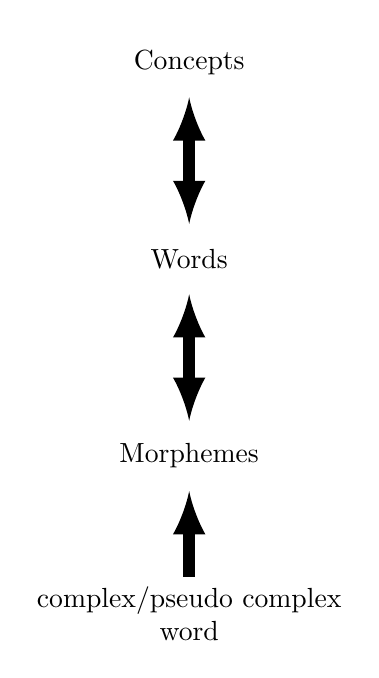
\begin{tikzpicture}
\node[n] (A) at  (0,7)	{Concepts};
\node[n] (B) at (0,4.5)	{Words};
\node[n] (C) at (0,2)	{Morphemes};
\node[n] (D) at (0,0)	{complex/pseudo complex\\ word};
\draw[dbl] (B)--(A);
\draw[dbl] (C)--(B);
\draw[spl] (D)--(C);
\end{tikzpicture}